\section{Construction inductive}

En logique mathématique, nous manipulons principalement des objets syntaxiques, signifiant que l'on considère des suites finies de termes définis par une grammaire inductive. On peut en général représenter de tels objets par des arbres : ainsi une proposition peut se dessiner comme un arbre où chaque nœud est un connecteur logique reliant des sous-formules. Nous en donnons un exemple dans la figure \ref{arbre}. Une définition par induction se ramènera, d'une façon ou d'une autre, à une structure d'arbre. Ainsi, comme toutes les définitions par inductions partagent des similarités, nous allons en introduire des outils permettant leur étude systématique, comme par exemple le raisonnement par induction structurelle. Nous utiliserons comme exemple dans cette section les entiers naturels et les arbres binaires, le premier par sa facilité (l'ensemble n'est constitué que de deux règles) et le second pour donner un exemple un peu plus général.

\includefig{Logique/chapitre_prop/proposition_arbre.tex}{Représentation de la proposition $\lnot P \implies Q$.}\label{arbre}

\subsection{Forme de Backus-Naur}

Nous utiliserons, pour définir un ensemble inductif, une grammaire dite en forme de Backus-Naur (abrégée BNF pour \textit{Backus-Naur Form}), dont le principe est de lister les constructeurs d'un ensemble inductif. Une BNF se présente de la façon suivante : $$ \alpha,\beta ::= \alpha_1\mid\alpha_2\mid\alpha_3\cdots$$ qui se lit :

\begin{itemize}[label=$\bullet$]
    \item Les éléments de l'ensemble que nous définissons seront notés $\alpha$ ou $\beta$.
    \item $\alpha_i$ est une règle permettant de construire un nouvel élément de notre ensemble inductif à partir d'éléments déjà construits. Chaque règle possède une arité associée, qui est le nombre d'arguments nécessaires pour construire un nouvel élément de l'ensemble inductif.
\end{itemize}

Nous allons maintenant donner deux exemples :

\begin{expl}[Entiers naturels]
    Les entiers naturels peuvent être définis par $$n,m ::= 0 \mid S n$$ ce qui signifie que $0\in \mathbb N$ et que si $n\in\mathbb N$ alors $S n \in\mathbb N$ (où le constructeur $S$ est l'opération successeur, c'est-à-dire la fonction $n \mapsto n+1$).
\end{expl}

\begin{expl}[Arbres binaires étiquetés par un ensemble]
    Soit $E$ un ensemble. On définit les arbres binaires étiquetés par $E$, notés $T(E)$ par la grammaire $$t,t' ::= \texttt{Nil}\mid \texttt{Node}(e,t,t')$$ où $e\in E$. Un arbre binaire est donc soit vide, soit un n\oe ud relié à un sous-arbre gauche et un sous-arbre droit.
\end{expl}

Remarquons que cette définition inductive peut se faire en introduisant des constructeurs : pour chaque règle de construction de notre grammaire, on associe une \og fonction \fg{} prenant un nombre fixé d'arguments inductifs pour générer un nouvel objet inductif.

\begin{expl}[Arbres binaires]\label{arbre_bin}
    On peut définir la règle précédente de la façon suivante : 
    \begin{itemize}[label = $\bullet$]
        \item il existe une constante $\texttt{Nil} \in T(E)$
        \item pour $e \in E$, il existe une fonction $\texttt{Node}_e : T(E)\times T(E)\to T(E)$
    \end{itemize}
\end{expl}

Si l'on s'abstrait des détails de notations, on peut définir une grammaire inductive comme un ensemble $C$ de constructeurs, avec une fonction $\alpha$ qui à un constructeur associe un entier, qui est le nombre d'arguments inductifs de la fonction permettant de construire un nouvel élément. 

\begin{defi}[Définition inductive]
    Comme dit précédemment, on appelle définition inductive un couple $\langle C,\alpha\rangle$ où $\alpha : C \to\mathbb N$. On appelle arité du constructeur $c$ l'entier $\alpha(c)$.
\end{defi}

Dans l'exemple \ref{arbre_bin} la définition inductive est donc $\langle \{0\} + E,\alpha\rangle$ où $\alpha(0) = 0$ et $\alpha(e) = 2$ pour $e\in E$.

\subsection{Ensemble défini par induction}

Nous avons vu la définition d'un ensemble par une grammaire, mais il convient encore de donner une construction d'un tel ensemble inductif. Il existe deux constructions dont on peut montrer qu'elles sont équivalentes : la construction \og par le bas\fg{} et la construction \og par le haut\fg{}. Nous n'étudierons ici que la construction par le bas, car celle-ci a le mérite d'être plus explicite.

\begin{defi}[Construction par le haut d'un ensemble inductif]
    Soit $\langle C,\alpha\rangle$ une définition inductive. A une telle définition on associe : 
    \begin{itemize}[label=$\bullet$]
        \item l'ensemble $I_0 = \{c\in C\mid \alpha(c) = 0\}$
        \item pour un ensemble $I_n$, l'ensemble $I_{n+1}=\{ (c,x) \in C\times {I_n^{\alpha(c)}}\mid \alpha(c) > 0\}\cup I_n$
    \end{itemize}

    On peut alors définit l'ensemble $\displaystyle{I = \bigcup_{n\in \mathbb N}I_n}$ associé à la définition inductive.
\end{defi}

\begin{rmk}
    Remarquons que, par construction, $I_n\subseteq I_{n+1}$. $I$ est alors l'ensemble des éléments qui appartiennent à un certain $I_n$. L'ensemble que nous avons construit est donc celui des éléments construits depuis une constante et une application finie de constructeurs.
\end{rmk}

Ces considérations nous mènent à donner le lemme suivant :

\begin{lem}[Lecture unique]
    Soit un ensemble inductif $E$ et $e\in E$. Alors soit $e$ est une constante (constructeur d'arité $0$) soit il existe $c,x$ tels que $e = (c,x)$ où $c$ est un constructeur d'arité $k$ et $x$ est un $k-uplet$ d'éléments de $E$. Ces cas sont tous exclusifs, au sens où les éléments $c$ et $x$ sont uniques.
\end{lem}

\begin{proof}
    Par définition, $e\in E$ signifie qu'il existe un $n\in \mathbb N$ tel que $e\in E_n$ (en notant $E_n$ les étapes de notre construction inductive). Dans ce cas, soit $N = \{m \in \mathbb N \mid e \in E_m\}$. Comme $n\in N$ et que $N$ est une partie de $\mathbb N$, il existe un plus petit élément, notons-le $m$. Si $m = 0$ alors $e$ est une constante. Si $m\neq 0$, alors $e = (c,x)$ où $c$ est un constructeur d'arité $k$ et $x$ est un $k$-uplet d'éléments de $E_{m-1}$ (la cas où $e\in E_{m-1}$ est impossible puisque $m$ est le minimum des étapes où $e$ est construit).

    Pour l'unicité, on remarque que si $(c,x) = e = (c',x')$ alors $c = c'$ et $x = x'$.
\end{proof}

\begin{rmk}
    Nous pouvons considérer un constructeur $c$ comme une fonction de son ensemble inductif dans lui-même (de la forme $c : E^{\alpha(c)} \to E$). Nous confondrons en général les deux objets. Remarquons aussi que chaque constructeur est injectif par construction.
\end{rmk}

Si toute cette construction semble alambiquée pour une notion aussi simple, avoir formulé de façon rigoureuse les définitions inductives permet de faire des preuves rigoureuses sur les structure inductives : c'est ce qu'on appelle une preuve par induction structurelle.

\begin{them}[Induction structurelle]
    Soit une propriété $P$ dépendant d'un paramètre $x$, sur un ensemble inductif $E$ généré par $\langle C,\alpha\rangle$. Alors $P$ est vraie sur $E$ tout entier si et seulement si $P(c)$ est vraie pour toute constante $c\in C$ et si pour $c$ d'arité $k$, pour tout $x_1,\ldots,x_k\in E$, $P(x_1)$ et $P(x_2)$ et $\ldots$ et $P(x_k)$ implique $P(c,(x_1,\ldots,x_k))$.
\end{them}

\begin{proof}
    Un sens est évident : si $P$ est vraie sur $E$, les deux conditions précisées sont vraies. Il suffit donc de prouver le sens réciproque. Procédons par récurrence sur $E_n$ :
    \begin{itemize}[label=$\bullet$]
        \item Par hypothèse, $P$ est vraie sur $E_0$.
        \item Si $P$ est vraie sur $E_n$, alors soit $e\in E_{n+1}$. Si $e\in E_n$, $P(e)$ est vraie. Par le lemme précédent, $e = (c,x)$ or chaque composante de $x$ est dans $E_n$ donc par hypothèse de récurrence, $P(x_1),\ldots,P(x_{\alpha(c)})$ sont vraies. On en déduit par hypothèse que $P(c,x)$ est vraie, donc $P$ est vraie sur $E_{n+1}$.
    \end{itemize}

    Donc par récurrence, $P$ est vraie sur $E$.
\end{proof}

De façon similaire, on peut définir une fonction uniquement grâce aux constructeurs.

\begin{them}[Définition d'une fonction par induction]
    Soit $E$ un ensemble défini par induction par $\langle C,\alpha\rangle$ et $F$ un ensemble quelconque. Supposons qu'à chaque constante $c_0$ on associe un élément $f_{c_0} \in F$, et qu'à chaque constructeur $c$ d'arité $a$ on associe une fonction $f_c : F^a \to F$. Alors il existe une unique fonction $f$ telle que $f(c_0) = f_{c_0}$ et pour chaque constructeur $c$, $f((c,(x_1,\ldots,x_a))) = f_c(f(x_1),\ldots,f(x_a))$.
\end{them}

\begin{proof}
    La preuve de l'existence et de l'unicité se fait par récurrence sur $E_n$ en prenant la proposition $P(n) =$ pour tout $e\in E_n$, il existe une unique fonction vérifiant ces conditions :
    \begin{itemize}[label=$\bullet$]
        \item Sur $E_0$, la seule fonction correspondante est $f_0 : c_0 \mapsto f_{c_0}$.
        \item Si on suppose définie une unique fonction $f_n : E_n \to F$, alors comme tout élément de $E_{n+1}$ est soit de la forme $(c,x)$ soit déjà dans $E_n$, un élément dans $E_n$ sera envoyé dans $F$ par $f_n$ (par unicité de $f_n$ partant de $E_n$) et un élément de la forme $(c,x)$ sera défini par la relation de récurrence : $f_{n+1}(c,x) = f_c(f(x_1),\ldots,f(x_n))$. Cette relation caractérise donc $f_{n+1}$ de façon unique.
    \end{itemize}
    D'où le résultat par récurrence.
\end{proof}

On peut représenter la définition inductive d'une telle fonction en disant que les diagrammes suivants, pour chaque constructeur $c$, commutent (dire qu'un diagramme commute signifie que deux chemins entre deux mêmes points sont égaux) :

\begin{center}
\begin{tikzcd}
    E\times \ldots \times E \ar[rr,"f\times \ldots \times f"] \ar[d,"c"] & & F\times\ldots\times F\ar[d,"f_c"]\\
    E \ar[rr,"f"] & & F
\end{tikzcd}
\end{center}

\begin{expl}[Liste]
    Soit $A$ un ensemble, on définit l'ensemble $\texttt{List}(A)$ par la grammaire $$ l::= \texttt{Nil}\mid \texttt{cons}(a,l)$$

    On notera par exemple $[\;]$ pour écrire la liste vide (plutôt que \texttt{Nil}) ou $[a,b,c]$ pour la liste construite par $\texttt{cons}(a,\texttt{cons}(b,\texttt{cons}(c,\texttt{Nil})))$, ou encore $a::[b,c]$.

    Définissons alors la fonction $|-|$ qui à une liste associe sa longueur. Par exemple $|[a,b,c]| = 3$. Pour cela, on définit la fonction par induction :
    \begin{itemize}[label=$\bullet$]
        \item $|[\;]| = 0$
        \item pour tout $a\in A$, $|a::l| = 1+|l|$.
    \end{itemize}

    Ainsi $|[a,b,c]| = 1 + |[b,c]| = 1 + 1 + |[c]| = 1 + 1 + 1 + |[\;]| = 3$.
\end{expl}

\begin{exo}[Les opérations dans $\mathbb N$]
    Définir les opérations add, mult et exp, définies naturellement par $\mathrm{add}(n,m) = n + m$, $\mathrm{mult}(n,m) = n \times m$ et $\mathrm{exp}(a,b) =  a^b$.\newline{}
    \textit{Indication : on peut définir une fonction à deux variables comme une fonction à une variable qui associe une fonction à une variable, et alors utiliser une définition inductive sur le premier argument.}
\end{exo}

\begin{exo}[Une meilleur récurrence]
    Remarquons qu'avec notre définition, si l'on définit $\mathbb N$ par le constructeur $0$ d'arité $0$ et le constructeur $s$ d'arité $1$, alors le principe d'induction pour définir une fonction de la forme $\mathbb N \to F$ consiste à donner un élément $c_0 \in F$ et une fonction $F\to F$. Montrer que ce principe de définition par induction permet de construire des fonctions définies par un élément $c_0\in F$ et une fonction $\mathbb N \times F \to F$. \textit{Indication : comme ce principe marche pour tout $F$, on peut chercher une fonction à valeur dans $\mathbb N \times F$ qu'on projettera ensuite sur $F$.}
\end{exo}

\begin{exo}\label{exo_arbre}
    En réutilisant la définition précédente des arbres binaires étiquetés par un ensemble $E$, construire une fonction donnant le nombre de n\oe uds de l'arbre (un arbre vide n'est pas un n\oe ud).
\end{exo}

Nous décrirons désormais nos ensembles inductifs directement par leur BNF. Nous supposerons donc assimilé le passage d'une grammaire à l'ensemble inductif qu'il décrit.

\subsection{Règle d'induction}

Nos résultats théoriques sont assez puissants pour définir beaucoup de choses, mais on peut remarquer que le formalisme qui leur est associé est assez lourd : nous allons donc définir une façon plus simple d'écrire nos définitions inductives. Pour construire un ensemble inductif, la grammaire en BNF est toute indiquée (elle est lisible et donne toutes les informations souhaitées). Cependant, pour définir une fonction par induction, nous allons donner un formalisme plus efficace, appelé règles d'induction. Comme nous l'avons dit, on peut classer nos constructeurs en deux sortes : ceux qui n'acceptent pas d'argument (les constantes) et les autres, qui acceptent un nombre précis d'arguments. Ainsi, si l'on veut définir une fonction $f : E \to F$ avec $E$ inductif, il suffit d'écrire une \og règle\fg{} permettant de passer d'un ensemble d'image à leur image par la fonction d'induction associée au constructeur.

\begin{expl}
    Supposons que l'on veuille définir $-\times 2 : \mathbb N \to\mathbb N$, il nous suffit d'écrire que $0\times 2 = 2$ et $(Sn)\times 2 = S(S(n\times 2))$.
\end{expl}

Mais dans le cas de structure inductives plus lourdes, il peut être avantageux d'avoir une présentation moins linéaire, c'est pourquoi l'on introduit la notion de règle d'induction.

\begin{defi}[Règle d'induction]
    Pour définir une fonction $f_c$ pour un constructeur $c$, on va utiliser la présentation suivante :
    \begin{center}
        \begin{prooftree}
            \hypo{a_1}
            \hypo{a_2}
            \hypo{\ldots}
            \hypo{a_n}
            \infer4{f_c(a_1,\ldots,a_n)}
        \end{prooftree}
    \end{center}
\end{defi}

\begin{rmk}
    Dans le cas d'une constante $c_0$, la règle s'écrit directement 
    \begin{center}\begin{prooftree} \infer0{f_{c_0}}\end{prooftree}\end{center}
\end{rmk}

On appelle souvent dérivation l'application d'une suite de règles d'inductions pour trouver l'image d'une fonction inductive, formant un arbre dont la racine est le résultat et les feuilles des constantes.

\begin{expl}
    Pour l'arbre $A$ suivant :
    \begin{center}
        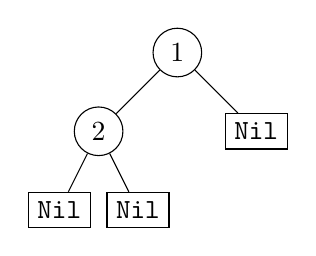
\begin{tikzpicture}
            \node[draw,circle] (A) at (0,0) {$1$};
            \node[draw,circle] (B) at (-1,-1) {$2$};
            \node[draw,rectangle] (C) at (1,-1) {\texttt{Nil}};
            \node[draw,rectangle] (D) at (-1.5,-2) {\texttt{Nil}};
            \node[draw,rectangle] (E) at (-0.5,-2) {\texttt{Nil}};
            \draw (A) -- (B) -- (D);
            \draw (A) -- (C);
            \draw (B) -- (E);
        \end{tikzpicture}
    \end{center}
    nous allons calculer son nombre de n\oe uds, en utilisant la fonction définie dans l'exercice précédent, dont on peut exprimer les règles d'induction de la façon suivante : 
    \begin{center}
        \begin{prooftree}
            \infer0{|\texttt{Nil}| = 0}
        \end{prooftree}
        \qquad
        \begin{prooftree}
            \hypo{|g| = k}
            \hypo{|d| = k'}
            \infer2{|\texttt{Node}(e,g,d)| = 1 + k + k'}
        \end{prooftree}
    \end{center}

    La dérivation est donc :
    \begin{center}
        \begin{prooftree}
            \infer0{|\texttt{Nil}| = 0}
            \infer0{|\texttt{Nil}| = 0}
            \infer2{|\texttt{Node}(2,\texttt{Nil},\texttt{Nil})| = 1 }
            \infer0{|\texttt{Nil}| = 0}
            \infer2{|A| = 2}
        \end{prooftree}
    \end{center}
\end{expl}


\begin{exo}
    Défnir les règles d'induction de la fonction $|-|$ sur les listes, associant à une liste sa longueur. \'Ecrire l'arbre de dérivation du calcul de $|[a,b,c]|$.
\end{exo}



\subsection{Relation inductive}

Intéressons-nous désormais aux relations entre objets inductifs. Comme précédemment, nous utiliserons des règles d'induction pour les définir (puisqu'une relation $\mathcal R$ peut être vue comme une fonction dans $\{0,1\}$), mais nous distinguerons deux types de prémisses : les prémisses du système formel et les prémisses \og meta\fg{}. Les premières sont celles qui interviennent directement dans les constructeurs de notre ensemble inductif, tandis que les deuxièmes sont des conditions que l'on peut dire extérieures à notre formalisme. Nous écrirons à côté de la règle les prémisses non syntaxiques (celles qui n'appartiennent pas au système formel). Attention cependant : nous nommerons souvent nos règles en donnant leur nom à droite de la barre, il faudra donc comprendre lorsqu'il y a une condition écrite à droite qu'elle est une prémisse non syntaxique, et lorsqu'il y a seulement un nom (par exemple $\to_e$) que c'est le nom de la règle.

\begin{expl}
    Nous allons définir le prédicat $P_k$ sur $\texttt{List}(\mathbb N)$ signifiant qu'une liste d'entiers possède un certain élément $k$ :
    \begin{center}\begin{prooftree}
        \hypo{}
        \infer1[$x = k$]{P_k(\texttt{cons}(x,l))}
    \end{prooftree}
    \qquad
    \begin{prooftree}
        \hypo{P_k(l)}
        \infer1{P_k(\texttt{cons}(x,l))}
    \end{prooftree}
    \end{center}
\end{expl}

\begin{exo}
    Montrer que $P_2([5,3,4,2,1,9])$ par un arbre de dérivation.
\end{exo}

\begin{rmk}
    On peut aussi définir des relations inductives mutuelles, par exemple un prédicat \og être pair\fg{} faisant appel à un prédicat \og être impair\fg{} faisant lui-même appel au premier prédicat (les deux ayant un cas de base), mais nous ne traiterons pas ce genre d'extension ici.
\end{rmk}

Donnons une définition de relation donnée par induction, car c'est un cas particulier qui nous sera utile.

\begin{defi}[Relation inductive]
    Soient $E,F$ deux ensembles. Soit un triplet $\langle C,\alpha,(D_c)_{c\in C}\rangle$ où $\alpha : C\to\nat, D_c : (E\times F)^{\alpha(c)}\to E\times F$ et $C$ est un ensemble. On dit que la relation $\mathcal R$ est définie par induction par ce triplet si $\mathcal R$ est la plus petite relation telle que pour tout $c\in C$, si pour tout $i \in\{0,\ldots,\alpha(c)\}, \mathcal R \langle x_i,y_i\rangle$ alors $\mathcal R(D_c(\langle x_1,y_1\rangle,\ldots,\langle x_{\alpha(c)},y_{\alpha(c)}\rangle))$. On note en général le triplet de la façon suivante : pour chaque $c\in C$, on écrit une règle de la forme
    \begin{center}
        \begin{prooftree}
            \hypo{\mathcal R(x_1,y_1)}
            \hypo{\mathcal R(x_2,y_2)}
            \hypo{\ldots}
            \hypo{\mathcal R(x_{\alpha(c)},y_{\alpha(c)})}
            \infer4[$c$]{\mathcal  R(D_c(\langle x_1,y_1\rangle,\ldots,\langle x_{\alpha(c)},y_{\alpha(c)}\rangle))}
        \end{prooftree}
    \end{center} avec $x_i,y_i$ non spécifiés, qu'il faut alors considérer comme quantifiée sur respectivement tout $E$ et tout $F$.
\end{defi}

\begin{exo}
    Montrer que si deux propositions sont stables par les règles définissant une relation inductive, alors l'intersection de ces propositions est aussi stable par ces règles. En déduire que la relation $\mathcal R$ définie par induction précédemment est l'intersection des propositions stables par les règles.
\end{exo}

\begin{exo}
    Montrer qu'une relation définie par induction par un ensemble de règles $\langle C,\alpha,(D_c)\rangle$ est non vide si et seulement s'il existe $c\in C$ tel que $\alpha(c) = 0$.
\end{exo}

\begin{rmk}
    Il arrivera que l'on écrive une règle dont les prémisses contiennent une ou des conditions qui ne sont pas de la forme $\mathcal R(x,y)$. Dans ce cas on peut considérer que l'on ajoute une règle de construction inductive pour chaque élément vérifiant cette prémisse et que le reste de la règle est paramétré par cet élément.
\end{rmk}

Nous pouvons maintenant réécrire notre théorème d'induction structurelle avec le formalisme des règles d'induction :

\begin{cor}[Preuve par induction]
    Soit une relation $\mathcal R$ entre deux ensembles $E,F$ générée par un ensemble de règles d'induction. Alors pour tout prédicat $P$ sur $E\times F$, pour montrer que $\mathcal R \subseteq P$ il suffit de montrer, pour chaque règle $c,\alpha(c),D_c$ définissant $\mathcal R$ la propriété suivante : pour tout $(x_1,\ldots,x_{\alpha(c)})\in P^{\alpha(c)}, P(D_c(x_1,\ldots,x_{\alpha(c)}))$, ce qui revient à montrer :
    \begin{center}
        \begin{prooftree}
            \hypo{P(x_1)}
            \hypo{P(x_2)}
            \hypo{\ldots}
            \hypo{P(x_{\alpha(c)})}
            \infer4[$c$]{P(D_c(x_1,\ldots,x_{\alpha(c)}))}
        \end{prooftree}
    \end{center}
\end{cor}

\begin{proof}
    C'est une conséquence directe du fait que $\mathcal R$ est définie comme la plus petite relation possédant cette propriété.
\end{proof}

